\section{Farbe}

\subsection{Was ist Farbe?}

\begin{itemize}
    \item \textbf{Physikalisch}, Lichtzusammensetzung, Elektromagnetischestrahlen
    \item \textbf{Physologisch}, Warnehmung und Interpretation
\end{itemize}

\textit{Farbe besteht aus:}

\begin{itemize}
    \item Farbton/Farbe
    \item Farbstich/Sättigung
    \item Helligkeit
\end{itemize}

\subsection{Farbe eines Objektes}

\textit{
    Ein Objekt nimmt Farbe auf und strahlt Farbe ab.
    Die Farbe des Objektes ist definiert durch die abgestrahlte
    Farbe.
}

\begin{itemize}
    \item Beleuchtung (Illumination)
    \item Reflektion (Reflection)
    \item Farbsignal (Color Signal)
\end{itemize}

\subsection{Licht besteht aus?}

\textit{
    Licht besitzt verschiedene Wellenlängen,
    Kombinationen dieser Frequenzen ergeben eine Farbe.
}

\begin{itemize}
    \item Sichtbares Licht (380mn - 780mn)
    \item Infrarot (780mn+)
    \item Ultraviolet (-380mn)
\end{itemize}

\textit{1nm = 10\AA (\AA ngström)} \\
\textit{1\AA = \o Atom}

\subsection{Das Auge}

\textit{
    Das Auge besteht aus; \textbf{Iris} (Muskel und Lichteinschränken),
    \textbf{Linse}, \textbf{Pupille} (Kontrolliert Iris) und \textbf{Retina}
    (Farb- und Lichtaufnahme am Rand des Auges)
} \\
\\
\textit{
    Die Retina besteht aus 75-100 $10^6$ Stäbchen (Lichtintensität) und
    6-7 $10^6$ Zäpfchen (Farbe). Die Forea ist der dichteste Platz.
}

\subsection{Wie sehen wir Farbe?}

\textit{Durch die 3 Arten von Zäpfchen:}

\begin{tabular}{ccccc}
    Kurz (S) & & Mittel (M) & & Lang (L) \\
    Blau     & & Grün       & & Rot \\
    440mn    & & 530mn      & & 560mn \\
    1        &:& 5          &:& 10 \\
\end{tabular}

\subsection{Wahrnehmung}

\textit{Grün 530mn wird am intensivsten wargenommen}

\textit{
    Die Helligkeitswahrnehmung zwischen Stäbchen und
    Zäpfchen ist unterschiedlich
}

\subsection{Farbsysteme}

\begin{itemize}
    \item \textbf{RGB} (Monitor, Spotligths,Pointilismus), \\
          additiv, C = (Rot, Grün, Blau)
    \item \textbf{CMY} (Drucken), \\
          subtraktiv, C = (Cyan, Magenta, Yellow)
    \item \textbf{CMYK}, CMY Mit Schwarz erweitert, \\
          K = min(Cyan, Magenta, Yellow) \\
          $C = C - K$, $M = M - K$, $Y = Y - K$
    \item \textbf{HSV}, \
          Farbton (Hue) / \
          Reinheit,Sättigung (Saturation) / \
          Intensität (Value)
    \item \textbf{YUV} (Alte Fernseher, UV = 1/4 Auflösung Farbkorrektur)\\
          Y = $0.229*R+0.587G+0.114*B$, \\
          U = $0.436(B-Y)/(1-0.114)$, \\
          V = $0.615(R-Y)/(1-0.299)$
    \item \textbf{CIE-Lab}, absolutes Farbsystem \\
          Achsensystem mit Helligkeit als Y-Achse und X/Z-Achse definieren Farbunterschiede
\end{itemize}

\subsection{Additives Farbsystem}

\textit{Farben additeren}
\textit{(1,1,1) = Weiss, (0,0,0) = Schwarz}

\subsection{Subtraktives Farbsystem}

\textit{Farben absorbieren}
\textit{(0,0,0) = Weiss, (1,1,1) = Schwarz}

\subsection{Farben Konvertieren}

\textit{Zu Grau: $I = 0.229*R+0.587G+0.114*B$} \\

\textit{RGB <> CMY: }
$\begin{pmatrix} C \\ M \\ Y \end{pmatrix} =
\begin{pmatrix} 1 \\ 1 \\ 1 \end{pmatrix} -
\begin{pmatrix} R \\ G \\ B \end{pmatrix}$ \\

\textit{HSV <> RGB: }\\
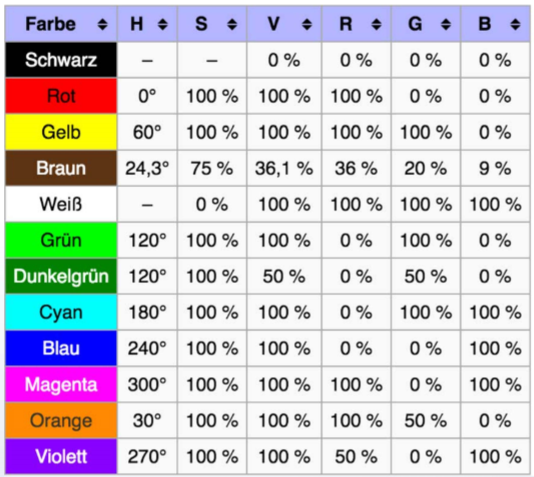
\includegraphics[width=0.4\textwidth]{assets/hsv-rgb.png}

\subsection{Gamma Korrektur}

\textit{
    Erreichen von gleichmässiger Verteilung der Helligkeit / Kontrast.
    Das Empfinden der Helligkeit ist nicht linear.
} \\
\\
\textit{
    Korrektur der Helligkeit des Bildes mit Gamme Wert. Wichtig für Bildschirme einstellen.
    Beim einstellen der Monitore Grauwerte mit echten Werten vergleichen (Gamma Test Pattern).
}

\subsection{Normfarbtafel}

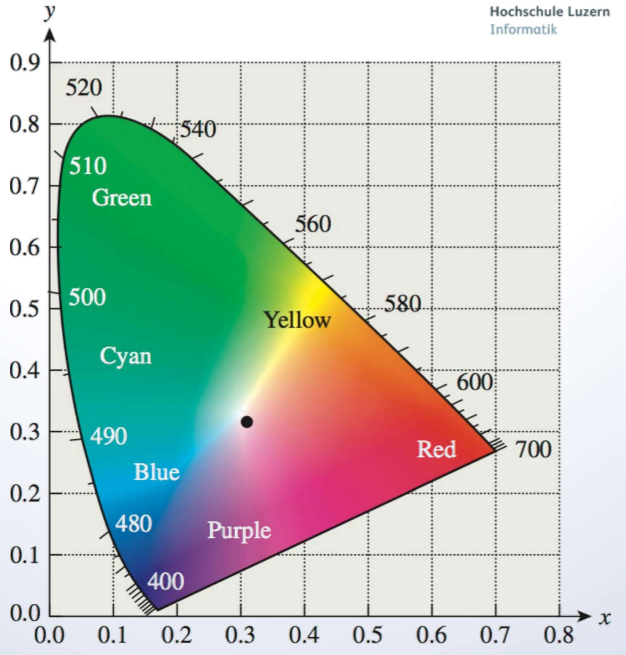
\includegraphics[width=0.4\textwidth]{assets/color-cie.png}

\subsection{Helligkeitswahrnehmung}

\textit{Helligkeit wird logarithmisch wahrgenommen, Webers Law}

$\frac{\Delta I}{I} = C$ \\
$\log (I + \Delta I) - \log(I) = Const$

\subsection{Nibs (Lichtdichte)}

\textit{
    Gibt Helligkeitsdichte für Auge an. 10nits werden stärker wargenommen denn 100nits.
    Heisst, weniger Licht wird stärker wargenommen.
}

\subsection{Mach bending}

\textit{
    Optische Illusion, bei zwei verschiedenen Grauwerten nebeneinander
    unterschieden sich diese vermeitlich stärker.
}

\subsection{Farbtäschung}

\textit{
    Farbe wird abhängig durch Umgebung anderst wargenommen
    (Dunkler, Heller). Optische Illusionen
}

\subsection{HD,UHD,UK}

\textit{Unterscheiden sich durch Pixelauflösung.}

\subsection{Was ist HDR?}

\textit{
    \textbf{High Dynamic Range}, speichert zusätzlichen Wert um
    Helligkeitsunterschiede besser unterschieden zu können
    (RGB-Pixelwerte propertianal zum Licht).
    Detailreichere dunkel und helle Spots, weniger Verlust
    durch Farben mit weniger Helligkeitsunterschiede.
}

\subsection{Begriffe}

\begin{tabular}{r|l}
    \textbf{Natürliches Licht}  & Gemisch aus verschiedenen \\
                                & Lichtwellen / Frequenzen \\
    \textbf{Spektralfarben}     & reine Farbfrequenz; Alle Farben \\
                                & am Rand des CIE-Farbsystems \\
    \textbf{Spektrum}           & Alle Frequenzen und deren \\
                                & Verteilung \\
    \textbf{Spektralverteilung} & Charakterisiert die Farbe, definiert \\
                                & durch Frequenzen \\
                                & (Bsp. Verschiedenes Weiss) \\
    \textbf{Komplementärfarben} & Addieren ergeben Grau, \\
                                & gegenüberligende Farben im \\
                                & CIE-Farbsystem
\end{tabular}
